\chapter{Generative Taggers using Finite-State Machines}
\label{chap:fsm}
In this Chapter, I will present an implementation of HMMs using {\it
  weighted finite-state machines}. It is further investigated in
Publications \ref{pub:1} and \ref{pub:2}. The implementation allows
for extensions of the HMM model in the spirit of \cite{Halacsy2007}
who utilize label context in the emission model of an HMM. It also
allows for applying global grammatical constraints. I will first
present a short summary of the most important aspects of finite-state
calculus and then present the finite-state implementation of HMMs.

\section{Weighted Finite-State Machines}

\paragraph{Automata} Weighted Finite-state automata are a data
structure for representing algorithms that solve the decision problem
of some regular language. A string can be either accepted or discarded
by a an automaton with some weight. Typically, weights bear
resemblance to probabilities and if they are interpreted as
probabilities, an automaton defines a distribution over the set of
strings. 

Figure \ref{fig:np-fsm} presents a finite-state which recognizes a
subset of noun phrases in the Penn Treebank. It illustrates the key
components of a finite-state automaton $M$
\begin{enumerate}
\item A finite set of states $Q_M$ ($\{0,\ 1,\ 2,\ 3,\ 4\}$ in Figure \ref{fig:np-fsm}).
\item An alphabet $\Sigma_M$ (the POS labels in Penn Treebank in Figure \ref{fig:np-fsm}).
\item A unique initial state $I_M$ ($0$ in Figure \ref{fig:np-fsm}).\footnote{Some formulations allow for several initial states with initial weights. This does, however, not increase the expressiveness of the formalism.}
\item A set of final states $F_M = \{r_1, ..., r_m\} \subset Q_M$ with associated final weights ${\rm f}(r_i)$ ($\{2\}$ and $1.0$ in Figure \ref{fig:np-fsm}).\footnote{Alternatively, we could also specify a final weight for every state. Then the actual final states would be the ones wit non-zero weight.}
\item A transition function $\tau_M$, which specifies a, possibly empty, set $\tau_M(q,x) = \{(q_1,w_1),\ ...,\ (q_n,w_n)\}$ of target states and transition weights for each symbol $x\in \Sigma_M$ in each state $q \in Q_M$ (in Figure \ref{fig:np-fsm} the relation is represented by the arrows in the graph).
\end{enumerate}
\begin{figure}[!ftb]
\begin{center}
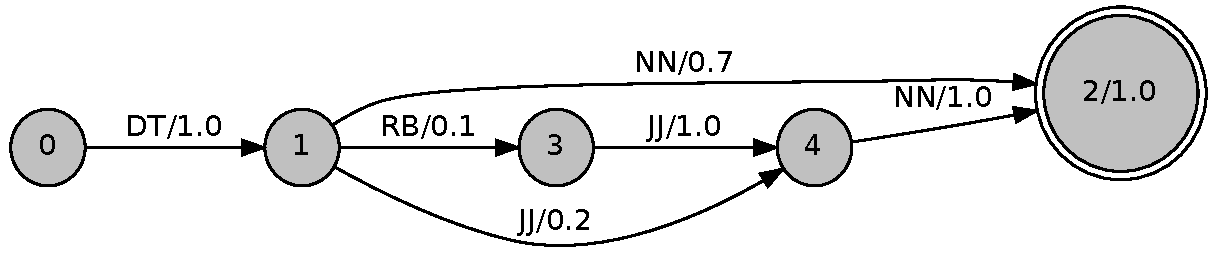
\includegraphics[scale=.7]{np}
\end{center}
\caption{A finite-state machine accepting a subset of the singular noun phrases in Penn Treebank.}\label{fig:np-fsm}
\end{figure}
When $\tau_M(a,q)$ is either empty or a singleton set for all $a$ and $q$, the automaton $M$ is called deterministic and I write $\tau_M(a,q) = (q_1,w_1)$ instead of $\tau_M(a,q) = \{(q_1,w_1)\}$.

\paragraph{Weight Semirings} Transition and final weights should form a
algebraical structure $\mathbb{K}$ called a semiring which is an abstraction of the
structure of positive real numbers under addition and multiplication. Consequently, two operations, addition $\oplus$ and
multiplication $\otimes$, are defined in $\mathbb{K}$. The addition operation should be
associative, commutative and have an identity element
$\mathbb{0}$. The multiplication operation should also be associative
and commutative. If it has an identity element, that element is
denoted by $\mathbb{1}$. The multiplication should distribute over the
addition \citep{Allauzen2007}.

As noted above, the prototypical example of a weight semiring is given by the positive real numbers together with the regular addition and multiplication of reals. This weight semiring, called the {\it probability semiring},\footnote{Even though the probability semiring is intended for representing probability distributions, weights cannot be restricted to $[0,1]$ the semiring has to be closed under addition.}  can be used to represent a probability distribution over the set of strings. In practice, this weight semiring is however rarely used. Because of numerical stability concerns, a logarithmic transformation $x \mapsto -log(x)$ is often applied to the weights and operations in the probability semiring. This gives the {\it log semiring}, where weights belong to $\mathbb{R}$, multiplication is given by $x \otimes y = x + y$ and addition by $x \oplus y = -\log(\exp(-x) + \exp(-y))$.

The addition operation of the log semiring $-\log(\exp(-x) + \exp(-y))$
is slow in practice. Moreover, $-\log(\exp(-x) + \exp(-y)) \approx y$
when $x \gg y$. Therefore, the addition operation in the log semiring
is often replaced by $x \oplus y = \min(x,y)$. This gives the {\it
  tropical semiring} which is the semiring used in this thesis.

I denote the transition weight of the transition leaving state $q_1$
with symbol $x$ and ending up in $q_2$ by $\w(\tau_M(q_1,x), q_2)$. As
a notational convenience, $\w(\tau_M(q_1,x), q_2) = \mathbb{0}$, if
there is no transition from $q_1$ to $q_2$. An automaton $M$ assigns a
weight to a path of states $p = (q_0,\ ...,\ q_{n+1})$, where $q_0 =
I_M$ and $q_n \in F_M$, and a string $s = s_1...s_n \in
\Sigma_M^{n}$. The weight is $\w_M(s,p)$ is given by Equation
\ref{eq:path-weight}. The total weight $\w_M(s)$ assigned to string
$s$ by automaton $M$ is given by Equation \ref{eq:string-weight}
\begin{equation}
\w_M(s,p) =
{\rm f}(q_{n+1})\otimes \bigotimes_{i = 0}^n \w_M(\tau_M(q_i,s_i), q_{i+1})\label{eq:path-weight}
\end{equation}

\begin{equation}
\w_M(s) =
\bigoplus_{p \in Q_M^{n+1}} \w_M(s,p) \label{eq:string-weight}
\end{equation}

\paragraph{Closure Properties} It is well known that regular languages
are closed under many unary and binary operations: union, negation,
concatenation and reversion \citep{Sipser1996}. Similarly, the class
of weighted finite-state machines is closed under these operations and
efficient algorithms for computing these operations exist. Table
\ref{tab:fs-algebra}, summarizes the properties of these algorithms.

\paragraph{N-Best}

\paragraph{Optimization} As stated above, a finite state machine where
each symbol and state is associated to maximally one transition is
called deterministic. It is well known that every finite-state machine
corresponds to a deterministic machine and this holds for weighted
finite-state machines as well \citep{Mohri2002}. A determinization
algorithm can be applied to any weighted finite-state machine in order
to produce a deterministic machine which accepts exactly the same set
of weighted strings as the original machine.

\begin{table}[!ftb]
\begin{center}
\begin{tabular}{lll}
Operation & Symbol & Definition \\
\hline
Power & $M^n$ & $\w_{M^n}(s) = \bigoplus_{s_1 ... s_n = s} \w_{M}(s_1) \otimes ... \otimes \w_{M}(s_n)$\\ 
Closure & $\bigoplus_{n = 0}^\infty M^n$ &  \\
Union & $M_1 \oplus M_2$ & $\w_{M_1 \oplus M_2}(s) = \w_{M_1}(s) \oplus \w_{M_2}(s)$\\ 
Concatenation & $M_1.M_2$ & $\w_{M_1.M_2}(s) = \bigoplus_{s_1s_2 = s} \w_{M_1}(s_1) \otimes \w_{M_2}(s_2)$\\
Intersection & $M_1 \cap M_2$ & $\w_{M_1 \cap M_2}(s) = \w_{M_1}(s) \otimes \w_{M_2}(s)$ \\
Composition & $M_1 \circ M_2$ & $\w_{M_1 \circ M_2}(s{\rm :}t) = \bigoplus_{r} \w_{M_1}(s{\rm :}r) \otimes \w_{M_2}(r{\rm :}t)$\\
\end{tabular}
\caption{A selection of operators for weighted finite-state machines
  given by
  \cite{Allauzen2007}.}\label{tab:fs-algebra}
\end{center}
\end{table}

%\paragraph{Transducers} Weighted finite-state automata solve the
%decision problem of regular languages with associated weights. In
%addition to this, a weighted finite-state transducer associates
%strings with a set of output strings. A WFST represent a {\it rational
%  relation} of strings. Whereas weighted automata can be seen as
%language models which weight each string, weighted transducers
%resemble analyzers or sequence labeling systems which output. Figure
%\ref{fig:np-fst} demonstrates this. It is a weighted analyzer for a
%few simple English noun phrases.

%The key difference between automata and transducers is the transition
%function. Unlike the transition function of an automaton, the
%transition function $\tau_M$ of a transducer $M$ maps a state $q$, an
%input symbol $x \in \Sigma_M$ and an output symbol $y \in T_M$ to a
%set of target states $\tau_M(q,x,y) \subset Q_M \times
%\mathbb{K}$. The sets $\Sigma_M$ and $T_M$ denote the input and output
%alphabet of the transducer $M$. Some transitions can lack an input or
%output symbol. A special empty string symbol $\epsilon$ is used to
%denote these. The input symbol of a transition therefore belongs to
%$\Sigma_M \cup \{\epsilon\}$ and the output symbol to $T_M \cup
%\{\epsilon\}$.

%The definition of the weight assigned by a transducer $M$ to paths and
%strings is very similar as in the case of automata. Given a path of
%states $p = (q_1,\ ...,\ q_{n+1})$, where $q_1 = I_M$ and $q_{n+1} \in
%F_M$, a sequence of pairs $u = ((s_1,t_1), ..., (s_n, t_n))$, where
%$x_i \in \Sigma_M \cup \{\epsilon\}$ and $y_i \in T_M \cup
%\{\epsilon\}$, the weight assigned to the path and pair sequence
%$\w_M(u,p)$ is given by Equation \ref{eq:fst-path-weight}. 

%Next, we will define the weight assigned to a string pair. Let $s \in
%\Sigma_M^*$ and $t \in T_M^*$, then a correspondence of $s$ and $t$ is
%a sequence of pairs $u = ((s_1,t_1), ..., (s_n, t_n))$, where $s_i \in
%\Sigma_M \cup \{\epsilon\}$, $t_i \in T_M \cup \{\epsilon\}$,
%$s_1...s_n$ equals $s$ except for some interleaved epsilons and the
%same holds for $t_1...t_n$ with respect to $t$. In this thesis I will
%assume that none of the pairs $(s_i,t_i)$ consists of two $\epsilon$
%symbols. This means that two strings $s$ and $t$ have only a finite
%number of correspondences. This simplifies the definition of the
%weight of a string pair. Let $c(s,t)$ be the finite set of
%correspondences of $s$ and $t$. Then the weight assigned to string
%pair $s{\rm : }t$ by transducer $M$, $\w_M(s{\rm :}t)$ is given by
%equation \ref{eq:fst-string-pair}.

%\begin{equation}
%\w_M(u,p) =
%{\rm f}(q_{n+1})\otimes \bigotimes_{i = 0}^n \w_M(\tau_M(q_i,x_i,y_i), q_{i+1}%)\label{eq:fst-path-weight}
%\end{equation}

%\begin{equation}
%\w_M(s{\rm :}t) =
%\bigoplus_{u \in c(s,t)} \bigoplus_{p \in Q_M^{|u| + 1}} \w_M(u,p) \label{eq:f%st-string-pair}
%\end{equation}

%\paragraph{Composition} Two transducers $M$ and $N$ represent weighted
%relations, $R_M$ and $R_N$ repsectively, between strings. It is
%possible to construct a weighted finite-state transducer which
%implements the relation $R_M \circ R_N$. The definition of this
%composition transducer $M \circ N$ is given in Table
%\ref{tab:fs-algebra}. Composition is a very useful operation because
%it allows for factorization of string transformations into simpler
%sub-transformation.

%Automata can be seen as a formalization of the concept of
%algorithm. They represent a restricted type of algorithm in the sense
%that they can only operate on symbol strings and they only operation
%they perform is to accept or reject a string. Although, this might
%sound quite restrictive, it turns out that most computational problems
%can be formalized as such {\it decision problems} involving only
%acceptance or rejection of symbol strings.

%Every automaton is associated with a {\it formal language} which is a
%(possible infinite) set of finite strings from the set of all strings
%of some finite alphabet. The automaton solves the decision problem of
%this language, i.e. accepts exactly those strings that belong to the
%language. {\it Weighted formal languages} are an extension to the
%concept of formal language, where each string should be assigned a
%weight. If the weights can be interpreted as probabilities, a weighted
%formal language over an alphabet $\Sigma$ can be seen as a probability
%distribution over the set of strings of the alphabet. However, this is
%not always possible because all weights cannot be interpreted as
%probabilities.

%Several well know classes of algorithms exist. The most famous ones
%are Turing machines which, in a sense, subsume all existing automata
%\cite{?}. In this thesis I have, however, utilized another class of
%automata, Finite-state machines. They are more restricted than Turing
%machines or another well know class, stack automata, because they
%utilize only a finite amount of memory. All real world implementations
%of automata of course utilize only a finite amount of memory.

%The restriction on memory limits the set of problems that finite-state
%machines can solve. However, at the same time it allows for a rich
%algebra which allows one to combine finite-state machines to produce
%new finite-state machines.

%The machine in Figure \ref{fig:np-fsm} accepts sequences of Penn
%Treebank labels which correspond to singular noun phrases that can
%have an adjective attribute (JJ) with an optional adverb (RB)
%expressing degree.

%Typically finite-state machines are represented as state transition
%graphs. An example is given in Figure \ref{fig:np-fsm}. The machine
%has a set of numbered {\it states} (0, 1, 2, 3 and 4) and {\it
%  transitions} from one state to another. The transitions are labeled
%using symbols from a finite alphabet (e.g. NN) and weights from a {\it
%  weight semiring}, when the machine is weighted. The weight semiring
%in this example is the {\it probability semiring} \cite{Allauzen2007}
%where weights are probabilities that can be added and multiplied in
%the usual fashion.

%Operation starts in the designated {\it start state} (0 in Figure
%\ref{fig:np-fsm}) and it has to end in a {\it final state} (2 in
%Figure \ref{fig:np-fsm} marked with a double ring). A string is
%accepted, if and only if there is a sequence of transitions leading
%from the start state to a final state where the symbols in the
%transition labels spell out the input string and the product of the
%weights along the path is non-zero. For example the machine in Figure
%\ref{np-fsm} accepts the string ``DT NN'' with weight 0.7 but rejects
%``DT JJ'' because the string inds when the machine is in state 4 but
%that is not a finite state.

%There may be several or no {\it accepting paths} for a given
%string. If there are several paths for some string, the machine is
%called {\it ambiguous}. More generally, a machine is called {\it
%  non-deterministic} if some state has several out-going transitions
%with the same label. Trivially, ambiguous machines are
%non-deterministic. In the case of ambiguous machines, the weight of a
%string is the sum of the weights of all of its accepting paths or zero
%if there are no accepting paths.


%\paragraph{Weighted formal languages} Formally, weighted languages are
%mappings $M : \Sigma^* \rightarrow \mathbb{K}$ from the set of
%arbitrary strings $\Sigma^*$ of some finite alphabet $\Sigma$ into
%some {\it weight semiring} $(\mathbb{K}, \oplus, \otimes, \mathbb{0},
%\mathbb{1})$ where $\mathbb{K}$ is a set of weights, $\oplus$ and
%$\otimes$ are addition and product operators for weights and
%$\mathbb{0} \in \mathbb{K}$ and $\mathbb{1} \in \mathbb{K}$ are the
%additive and multiplicative identity.

%\paragraph{Weight semirings} As mentioned above, the weight semiring
%in Figure \ref{fig:np-fsm} is the probability semiring, where weights
%belong to the set of non-negative reals $[0, \infty)$ and addition and
%product are given by the regular real addition and product
%operations. Even though probabilities reside in $[0,1]$, the addition
%of probabilities can result in quantities that are larger than
%$1$. Because finite-state algebra does include operations that add
%probabilities, the weight set needs to include all non-negative reals.

%The general weight semiring $(\mathbb{K}, \oplus, \otimes, \mathbb{0}, \mathbb{1})$ is an abstraction of the probability semiring. The set $\mathbb{K}$ is an arbitrary set but the operations $\oplus \rightarrow \mathbb{K} \times \mathbb{K} \rightarrow \mathbb{K}$ and $\oplus \rightarrow \mathbb{K} \times \mathbb{K} \rightarrow \mathbb{K}$ need to satify the following requirements \cite{Allauzen2007}
%\begin{enumerate}
%\item $(\mathbb{K}, \oplus, \mathbb{0})$ is a commutative and associative monoid.
%\item $(\mathbb{K}, \otimes, \mathbb{1})$ is an associative monoid.
%\item $\otimes$ distributes with respect to $\oplus$.
%\item $\mathbb{0}$ is the annihilator of $\otimes$.
%\end{enumerate}
%If $\oplus$ is a group operation, the semiring is in fact a ring. Many
%useful weight semirings are, however, not rings. Often the semiring
%$(\mathbb{K}, \oplus, \otimes, \mathbb{0}, \mathbb{1})$ is denoted
%simply as $\mathbb{K}$. Paralleling the regular sum notation $\Sigma_{i \in I} x_i$ and product notation $\prod_{i\in I} x_i$, I use the notations $\bigoplus_{i \in I} x_i$ and $\bigotimes_{i \in I} x_i$, where $I$ is a denumerable set.\footnote{Infinite sums and products are not defined in all semi rings, for example the probability semiring. In this case, it is often possible to augment the semirings with an infinity element $\infty$. This problem does not often cause problems in practice and will not be examined further.} Specifically $\oplus_{i \in \emptyset} x_i = \mathbb{0}$ and $\otimes_{i \in \emptyset} x_i = \mathbb{1}$.

%Weights in the probability semiring and the addition and product operations have an intuitive interpretation but from a practical point of view the probability semiring is sub optimal. The biggest drawback is that repeated multiplication of probabilities gives rise to very small quantities and under-flow becomes a problem. Therefore, the so called {\it logarithmic semiring} is more commonly used. It can be derived by applying a logarithmic transformation $x \mapsto -\log(x)$ to the weights and operations in the probability semiring. 

%In the logarithmic semiring, numerical under-flow is not a problem but
%the addition operation given by $x \oplus y = -\log(\exp(-x) +
%\exp(-y))$ is resource intensive. Therefore, another semiring, the
%{\it tropical semiring}, is often used. The addition operation in the
%tropical semiring is given by $x \oplus y = \min(x,
%y)$. Computationally, this operation is light. A theoretical
%motivation is given by the fact that $\min$ preserves the magnitude of
%the sum although not its exact value. In practice, this is often
%sufficient \cite{?}. All machines in this thesis use tropical
%weights.

%\paragraph{Weighted finite-state automata} Formally, a weighted
%finite-state automaton of weight semiring $\mathbb{K}$ is a structure
%$M = (\Sigma, Q, q_0, \rho, E)$ where
%\begin{enumerate}
%\item $\Sigma$ is a finite symbol set (also called an alphabet).
%\item $Q$ is a finite set of states.
%\item $q_0 \in Q$ is the unique start state.
%\item $\rho: Q \rightarrow \mathbb{K}$ is the final weight map.
%\item $T \subset Q \times (\Sigma \cup \{\epsilon\}) \times Q \times
%\mathbb{K} $ is a finite set of transitions.
%\end{enumerate}

%The final weight map $\rho$ associates each state $q \in Q$ with a final weight. The final states of $M$ are $\{q \in Q\ | \rho(q) \ne \mathbb{0}\}$.

%Each transition $x \in T$ consists of a source state $\s(x)$, an input symbol $\i(x)$, a target state $\t(x)$ and a weight $\w(x)$. The input symbol may be $\epsilon$ which denotes the empty symbol. For the single outgoing transition $x$ in state 4 in Figure \ref{fig:np-fsm}, the source state $\s(x) = 4$, the input symbol $\i(x) = {\rm "NN"}$, the target state $\t(x) = 2$ and the weight $\w(x) = 1.0$.

%A sequence of transitions $x_1, ..., x_n \in T$ is a {\it path}, if
% $\s(x_1) = q_0$ and $\t(x_{k-1}) = \s(x_k)$ for all $k$. As a special case, the empty
%sequence is also a path. The weight of path $p = (x_1, ..., x_n)$ is $\w_M(p) = ( \prod_{i = 1}^n \w(x_i) ) \otimes \rho(x_n)$ and the weight of the empty sequence is $\rho(q_0)$. A path $p$ is called successful when $\w_M(p) \ne \mathbb{0}$.

%Each path $p = (x_1, ..., x_n)$ is associated with a unique, possibly
%empty, string $s \in \Sigma^*$ such that there is a subsequence $j_i,
%..., j_m$ of $1, ..., n$ for which $i(x_{j_1}), ..., i(x_{j_m}) = s$
%and $i(x_{l}) = \epsilon$ whenever $l \notin \{j_1, ..., j_m\}$. If
%the path $p$ is associated with the string $s$, it is called a {\it
%  path of $s$}.

%The set of paths of a string $s$ is denoted $P_s$ and the weight
%assigned to $s$ by the automaton $M$ is $\w_M(s) = \bigoplus_{p \in
%  P_s} \w_M(p)$. When $P_s = \emptyset$, $\w_M(s) = \mathbb{0}$. The
%string $s$ belongs to the weighted language $L(M)$ accepted by $M$ if
%$L(M)(s) = \w_M(s) \ne \mathbb{0}$.

%\section{Finite-State Algebra}
%
%Finite-state machines use only a finite fixed amount of
%memory. Therefore, they cannot solve all computational problems. There
%is, for example, no finite-state machine which accepts only strings of
%prime number length. This can be proved using the pumping lemma of
%regular language \citep{Sipser1996} which are the languages whose
%decision problems finite-state automata can solve.
%
%Although the computational power of finite-state machines is limited,
%they are closed under a number of very useful operations which
%correspond to set theoretical operations of the languages recognized
%by the machines. The collection of these operations is called the {\it
%  finite-state algebra}.
%
%Table \ref{tab:fs-algebra} gives an overview of a number of well known
%finite-state operations.
%
%
%
%\section{Finite-State Transducers}
%Language processing frequently requires translation of one signal such
%as speech or text into another signal, for example text in another
%language in the case of machine translation or annotated text in the
%case of part of speech tagging. These do not seem like the kinds of
%processing tasks that finite-state machines can solve because, as we
%saw above, finite-state machines solve decision problems.
%
%Weighted Finite-state transducers are an extension of weighted
%finite-state automata. Whereas finite-state automata simply accept or
%reject a symbol sequence, finite-state transducers simultaneously
%output another symbol sequence.

%\begin{figure}
%\begin{center}
%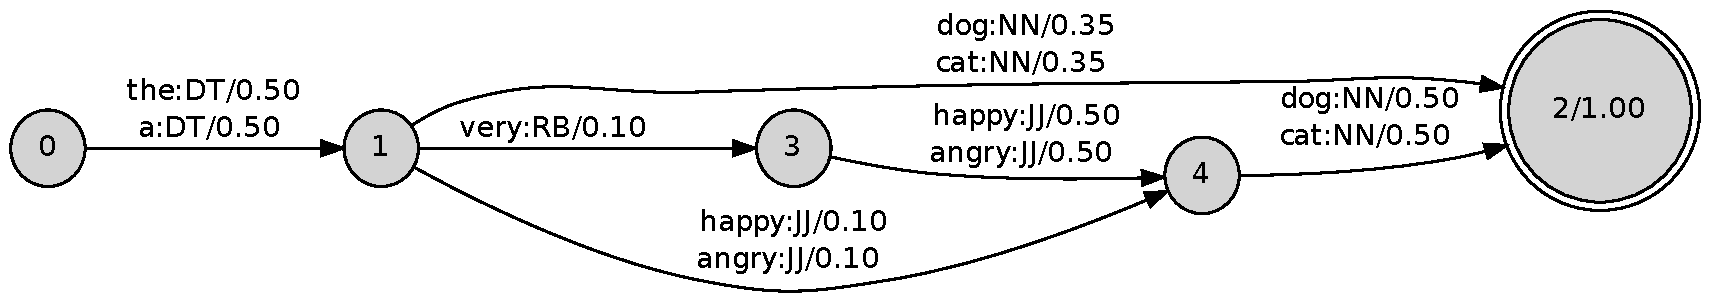
\includegraphics[scale=.5]{np_a}
%\end{center}
%\caption{A finite-state transducer that analyzes a subset of the singular noun% phrases in Penn Treebank.}\label{fig:np-fst}
%\end{figure}
%
%Formally, a weighted finite-state transducer of weight semiring
%$\mathbb{K}$ is a structure $M = (\Sigma, \Omega, Q, q_0, \rho, E)$ where
%\begin{enumerate}
%\item $\Sigma$ is a finite input symbol set (also called an input alphabet).
%\item $\Omega$ is a finite output symbol set (also called an output alphabet).
%\item $Q$ is a finite set of states.
%\item $q_0 \in Q$ is the unique start state.
%\item $\rho: Q \rightarrow \mathbb{K}$ is the final weight map.
%\item $T \subset Q \times (\Sigma \cup \{\epsilon\}) \times (\Omega \cup \{\epsilon\}) \times Q \times
%\mathbb{K} $ is a finite set of transitions.
%\end{enumerate}
%
%Transitions $e \in T$ are similar to transitions in automata but in
%addition to the input symbol $\i(e)$, they also contain an output
%symbol $\o(e)$. Paths of transitions are defined in the same way as
%paths for automata, however, paths of transducer transitions are
%associated with two strings -- an input and an output string. The
%input string of path $p = (x_1, ..., x_n)$ is the string $s_i =
%\i(x_1) ... \i(x_n)$ disregarding epsilons and the output string is
%$s_o = \o(x_1) ... \o(x_n)$ also disregarding epsilons. Path $p$
%itself is associated with the string pair $s = s_i \: s_o$. The set of
%paths associated with the input string of $s$ is $\P_i(s)$ and the set
%paths associated with of output string is $\P_o(s)$.
%
%The weight of path $p$ is defined in exaclty the same way as for
%automata 
%$$\w_M(p) = \Big( \prod_{i = 1}^n \w(x_i) \Big) \otimes \rho(x_n).$$
%
%A transducer $M$ can be viewed as a machine that maps input strings to
%sets of output strings with weights. Equivalently, it can be seen as a
%machine accepting string pairs $s = s_i \: s_o$ with some weight $\w_M(s)$. The
%weight $\w_M(s)$ given to string pair $s$ by transducer $M$ is defined 
%$$\w_M(s) = \bigoplus_{p \in \P_i(s) \cap \P_o(s)} \w_M(p)$$
%The defition takes into account the fact that there may be several
%alignments of input and output string giving the exact same string
%pairs. For example, $(\epsilon\:b, a\:b)$ and $(a\:b,\epsilon\:b)$
%represent the same string pair $a\:bb$.

\section{Finite-State Implementation of Hidden Markov Models} As seen
in Chapter \ref{chapter:hmm}, a generative HMM can be decomposed into
an emission model $p(x_i|y_i)$ of emissions $x_i$ given states $y_i$ a
transition model $p(y_{n+1} | y_1, ..., y_n)$, which models the
conditional distribution of a state $y_{n+1}$ given a state history
$y_1, ..., y_n$. As shown in Publications \ref{pub:1} and \ref{pub:2}
both of these can be compiled into weighted finite-state machines.

A generative HMM can be represented as a weighted finite-state machine
in several ways. The implementation presented in Publication
\ref{pub:1}, however, allows for enriching the emission model by
conditioning them on neighboring word forms and labels.

The main idea of the implementation discussed in Publication
\ref{pub:1} is to represent a labeled sentence as a string of word
form/label pairs as in Figure \ref{fig:lab-sent}. The emission and
transition models are implemented as weighted finite-state machines
which assign weights to such labeled sentences. Because of this
representation, both the emission model and transition model can
access information about the sequence of word forms and their
labels. Therefore, the emission and transition models can use more
information than in a regular HMM model. The sentence, emission and
different models are combined using the operations of finite-state
algebra.

In a normal HMM tagger, extension of the emission and transition model
requires changes to inference algorithms used by the tagger. In
contrast to a traditional HMM tagger, the finite-state tagger
presented in Publications \ref{pub:1} and \ref{pub:2} uses an n-best
paths algorithm for inference. This is a general algorithm which can
be applied on any model that can be represented as weighted
finite-state machine. Therefore, extending the emission and transition
models requires no changes to the inference procedure.

In this Section, I will discuss the implementation of a HMM model. In
the next Section, I will show how emission and transition models can
be extended.

\begin{figure}[!htb]
\begin{center}
\begin{tabular}{|l|l|l|l|l|l|l|l|}
\hline
The & DT & dog & NN & sleeps & VBZ & . & .\\
\hline
\end{tabular}
\caption{The representation of a labeled sentence as a single sequence.}\label{fig:lab-sent}
\end{center}
\end{figure}

\paragraph{Emission Model} Let $x = (x_1, ..., x_T)$ be a sentence and
let $Y_t = \{y_t^1, ..., y_t^n\}$ be the set of possible labels for
word $x_t$. Then we can construct a very simple finite-state machine
$X_t$ which recognizes the word $x_t$ and one of its possible labels
$y_t \in Y_t$ and assigns that combination a log weight corresponding
to the probability $p(x_t\cond y_t^i)$. As in the case of a regular HMM tagger,
$p(x_t\cond y_t)$ can be estimated from the training data. For OOV words,
we can use a guesser, for example the one presented in Chapter
\ref{chapter:hmm}.

As an optimization, only the most probable labels for each word can be
included in the emission model. However, it is completely possible to
include all labels for each word.

The individual emission machines $X_t$ can be combined into a sentence
model by concatenation as shown in Figure
\ref{fig:sentence-model}. The paths through the sentence model
correspond to the possible label assignments of sentence $x$.

\begin{figure}[!htb]
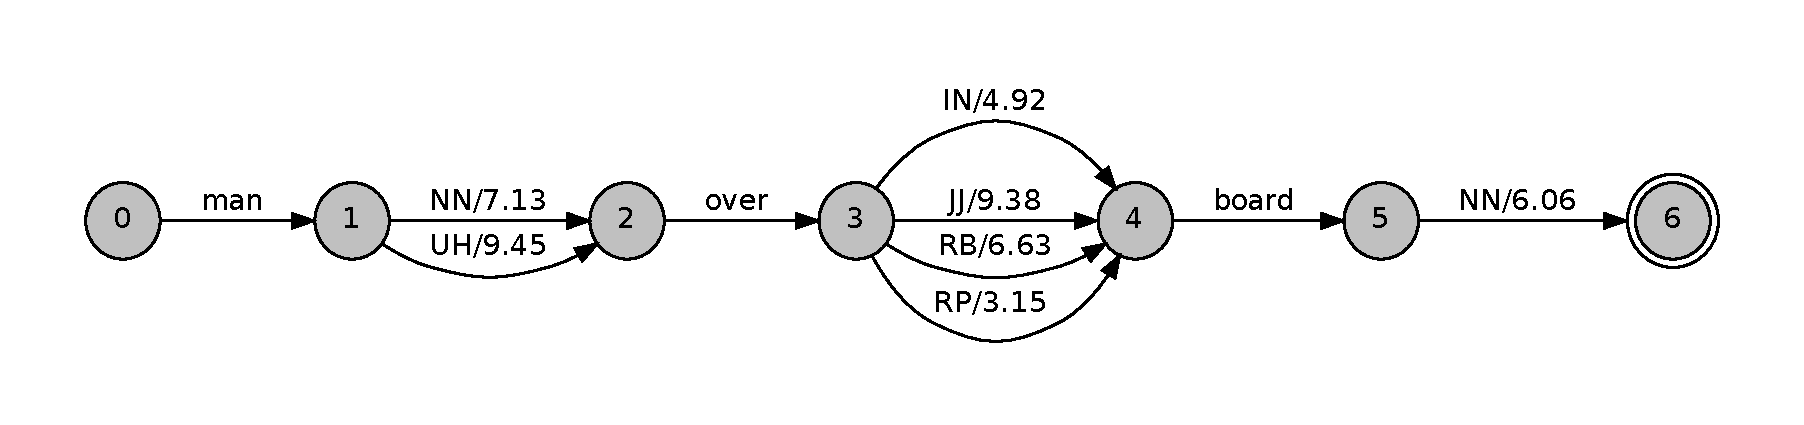
\includegraphics[scale=0.5]{sentence_model}
\caption{An example of a sentence model. The weights on the arcs are
  negative logarithms of emission probabilities. Only a subset of the
  possible labels are shown in the picture.}\label{fig:sentence-model}
\end{figure}

\paragraph{Transition Model} As stated above, Publications \ref{pub:1}
and \ref{pub:2} represent labeled sentences as a sequence of pairs
where each pair consists of a word form and a label. The transitions
model assigns weight to such sequences. I will explain the
construction of the transition model in three phases:
\begin{enumerate}
\item How to construct a model which assigns weight $-\log(p(y_{n+1}\cond
y_{1}, ..., y_{n}))$ to label n-gram $y_1, ..., y_{n+1}$.
\item How to extend the model to assign weight to an n-gram of word form/label pairs.
\item How to score an entire labeled sentence.
\end{enumerate}
The construction presented below will result in a number of
deterministic finite-state machines whose combined effect (the
intersection of the machines) corresponds to the n-gram model in a
standard HMM.

\paragraph{Scoring one label n-gram} The transition distributions $p(y_i\cond
y_{i - 1}, ..., y_{i - n})$ in an n-th HMM encodes the likelihood of
label sequences. I will first consider the problem of constructing a
machine which represents transitions weights for isolated label
n-grams. 

To emulate transitions weights in an HMM using finite-state calculus,
we can first compile a machine $T$ which accepts any sequence of $n+1$
labels $y_{1}, ..., y_{n+1}$. The weight assigned by the machine to
one of these paths can be estimated from a training corpus for the
sequences occurring in the corpus. Some form of smoothing is required
to score label n-grams missing from the training corpus. In
Publication \ref{pub:2}, a very simple form of smoothing is used. Each
n-gram not occurring in the training corpus will receive an identical
penalty weight $-\log(1/(N+1))$, where $N$ is the size of the training
corpus. Additionally, Publication \ref{pub:2} uses interpolation of
probability estimates of n-grams of different orders. More
sophisticated smoothing schemes could also be applied at the cost of
larger model sizes.

[WRITE ABOUT DETERMINIZATION AND MINIMIZATION]

If the machine $T$ is deterministic and has one path corresponding to
each label n-gram $y_1, ..., y_{n+1}$, where $y \in \mathcal{Y}$, each
non-terminal state in the machine will have $\mathcal{Y}$
transitions. Because $T$ encodes the weight $p(y_{n+1}\cond y_{1},
..., y_{n})$ for each label n-gram, it will have a large amount of
states when many label n-grams occur in the training corpus. It is
difficult to present a formal analysis of the size of $T$ as a
function of the number of distinct label n-grams in the corpus. An
example can, however, illustrate the number of states that are
typically required.

For the FinnTreeBank corpus, 8801 non-terminal states are required to
represent $T$ for $n=2$. As the corpus has $1399$ distinct
morphological labels, this translates to approximately 12 million
transitions. When using add one smoothing, most label n-grams will
have the same weight.

If the machine $T$ is deterministic and has one path
corresponding to each label n-gram $y_1, ..., y_{n+1}$, where $y \in
\mathcal{Y}$, each non-terminal state in the machine will have
$\mathcal{Y}$ transitions. Because $T$ encodes the weight
$p(y_{n+1}\cond y_{1}, ..., y_{n})$ for each label n-gram, it will
have a large amount of states when many label n-grams occur in the
training corpus. It is difficult to present a formal analysis of the
size of $T$ as a function of the number of distinct label n-grams in
the corpus. An example can, however, illustrate the number of states
that are typically required.

For the FinnTreeBank corpus, 8801 non-terminal states are required to
represent $T$ for $n=2$. As the corpus has $1399$ distinct
morphological labels, this translates to approximately 12 million
transitions. When using add one smoothing, most label n-grams will
have the same weight.

In order to, reduce the size of the model, so called {\it failure
  transitions} can be used \citep{someone}. A failure transition in a
state $q$, will match any symbol which does not have another outgoing
transition in $q$. The failure transitions will go to sink states,
which encode the penalty weight for unseen label n-grams.  Using
failure transitions, most states will not have $|\mathcal{Y}|$
transitions. Because of data sparsity, most state will in fact have
only a few outgoing transitions. Figure \ref{fig:fail_t} illustrates a
bigram model with failure transitions.

\begin{figure}
\begin{center}
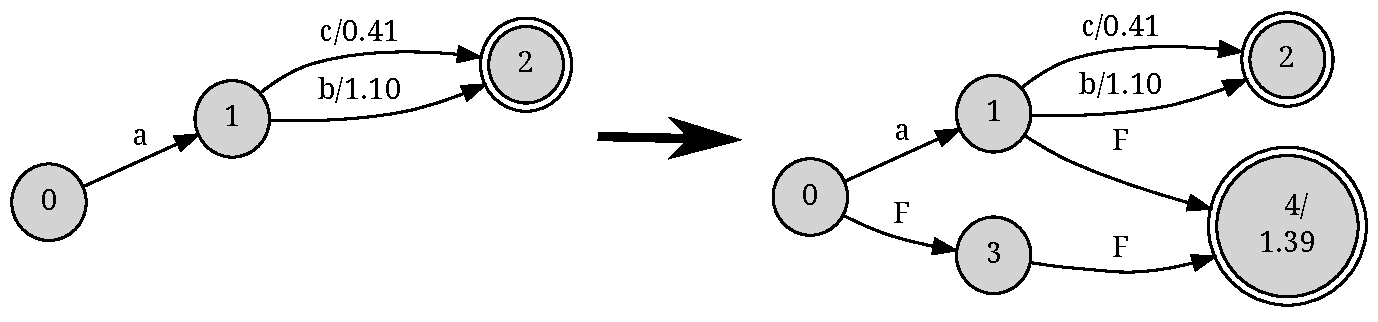
\includegraphics[scale=0.5]{fail_t}
\caption{Failure transitions (with symbol F) are added to a bigram model.}\label{fig:fail_t}
\end{center}
\end{figure}

I will now outline the procedure to compute a machine with failure
transitions in the general case. We first need an auxiliary
definition. For a state $q \in Q_T$, let $n(q)$ be the length of the
shortest symbol string required to reach state $q$ from the initial
state $q_0$.  Now, given a machine $T$ that recognizes every label
n-gram occurring in the training corpus, a corresponding machine $T_f$
with failure transitions can be computed.

\begin{enumerate}
\item $n+1$ new sink states are added: $Q_{T_f} = Q_T \cup \{s_1, ...,
  s_{n+1}\}$. The state $s_{n+1}$ is final and its final weight is the
  penalty weight for unseen n-grams.
\item A failure symbol is added: $\Sigma_{T_f} = \Sigma_T \cup \{f\}$, where $f \notin \Sigma_T$.
\item $\tau_{T_f}(q,a) = \tau_T(q,a)$ for all $q \in Q_T$ and $a \in \Sigma_T$. 
\item $\tau_{T_f}(s_1,f) = \{(s_{i+1}, \mathbb{1}\}$ for $i <= n$.
\item Failure transitions are added: $\tau_{T_f}(q, f) = \{(s_{n(q)}, \mathbb{1})\}$.
\end{enumerate}

\paragraph{Adding word forms} The current transition model scores
label n-grams. However, because we represent labeled sentences as
sequences of word form/label-pairs, we need to include word forms in
the model. This can be accomplished by adding a number of new states
and failure transitions to the model. When implementing a standard HMM
tagger, the added failure transitions will simply skip word
forms. Figure \ref{fig:fail_t_wf} demonstrates the construction for
the transition model in Figure \ref{fig:fail_t}.

\begin{figure}[!htb]
\begin{center}
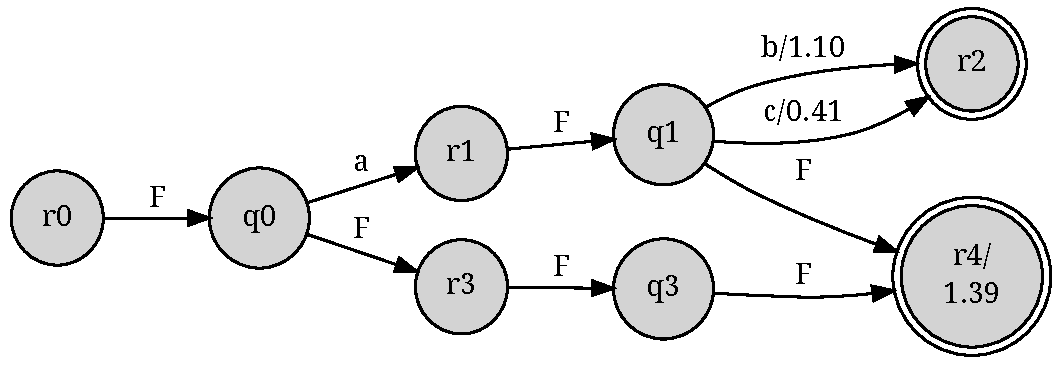
\includegraphics[scale=0.5]{fail_t_wf}
\caption{The transition model in Figure \ref{fig:fail_t} is augmented
  with failure transitions and states in order to be able to handle
  word forms.}\label{fig:fail_t_wf}
\end{center}
\end{figure}

We construct a new machine $T_w$ which accepts n-grams of word
form/label-pairs. Let $Q_{T_f} = \{q_0, ..., q_k\}$, then $Q_{T_w} =
Q_{T_f} \cup {r_0, ..., r_k}$, where $r_i \notin Q_{T_f}$. Let $r_0$
be the start state of $Q_{T_f}$ and let $F_{T_f} = F_{T_w}$. The
transitions function $\tau_{T_w}$ is defined in the following way.

\begin{enumerate}
\item $\tau_{T_w}(r_i,f) = \{(q_i,\mathbb{1})\}$.
\item $\tau_{T_w}(q_i,x) = \{(r_j,w)\}$ for all $x \in \Sigma_{T_w}$, if $\tau_{T_f}(q_i,x) = \{(q_j,w)\}$.
\end{enumerate}

Consider two states $q_1,q_2 \in Q_M$, in a machine $M$ with failure
transitions. Failure transitions in $q_1$ and $q_2$ may match a
different set of symbols. For example, If $q_1$ has a transition with
symbol $a \in \Sigma_M$ and $q_2$ does not, then $a$ will match the
failure transition in $q_2$ but it will not match the failure
transition in $q_1$. This is a problem when the determinization
algorithm is applied to $M$ because determinization joins states.
State joining may change the language accepted by $M$ and the
weights assigned to strings. 

It is highly desirable that the transition model of the finite-state
implementation of an HMM tagger is deterministic because of reduced
tagging time. However, as noted above, we cannot use standard
determinization with machines which have failure
transitions. Therefore, the construction presented below will produce
deterministic machines without resorting to determinization.

\paragraph{Scoring a sentence} We will now see how the transition
model for scoring an isolated label n-gram can be extended for scoring
an entire sentence. Given the machine $T_w$ which scores one n-gram,
we can form the Kleene closure of $T_w$. Since $M_n$ is an acyclic
machine accepting strings of equal length (that is $2n$: $n$ word
forms and $n$ labels), we can easily compute a deterministic Kleene
closure $T_{w}^*$ of $T_w$ by re-directing transitions going to final
states into the initial state\footnote{It can easily be seen that this
  construction fails if the machine accepts strings of unequal
  lengths.}
\begin{enumerate}
\item $\Sigma_{T_w^*} = \Sigma_{T_s}$. 
\item $Q_{T_w^*} = Q_{T_w} - F_{T_w}$.
\item $F_{T_w^*} = \{q_0\}$ and $f(q_0) = \mathbb{0}$.
\item $\tau_{T_w^*}(a,q) = \{(q', w)\}$, if $\tau_{T_w}(a,q) = \{(q',
  w)\}$ and $q'\notin F_{T_w}$.
\item If $\tau_{T_w}(a,q) = \{(q', w)\}$ and $q' \in F_{T_w}$, then
  $\tau_{T_w^*}(a,q) = \{(q_0, w + f(q'))\}$.
\end{enumerate}

The machine $T_{w}^*$ will score entire labeled sentences, however, it
only scores some of the trigrams in the sentence, namely, the ones
starting at positions divisible by $n+1$. Fortunately we can form $n +
1$ machines $T_0$ ... $T_n$ which will score all remaining
n-grams. Let $T_0 = T_{w}^*$ and let $T_{i+1} = F.F.T_i$. Intuitively
each $T_i$ will skip $i$ word form/label-pairs.

The final scoring of all possible labeled sentences, corresponding to
an input sentence $x$, is accomplished by intersecting the sentence
model $X$ and each of the $T_i$ using an intersection algorithm which
handles failure symbols correctly. In Publications \ref{pub:1} and
\ref{pub:2} a parallel intersection algorithm \citep{Silfverberg2009},
however, this is not actually required. The intersections can be
performed sequentially.

\paragraph{Smoothing} As observed in Chapter \ref{chapter:hmm}, a
second order model usually gives the best results in morphological
tagging. However, a pure second order model suffers from data sparsity
which degrades it performance. This can be avoided using smoothing. In
Publications \ref{pub:1} and \ref{pub:2}, smoothing is accomplished by
using first and zeroth order transition models in addition to the
second order transition model. To get the combined effect of all
models, each of them is intersected with the sentence model.

Usually, for example in \cite{Brants2000}, the transition
probabilities $p(y_i|y_{i-1}, y_{i-2})$ are a linear interpolation of
the probability estimates $\hat{p}$ for different orders as shown in
equation \ref{eq:ip}. \cite{Brants2000} sets the values for $\alpha_i$
using deleted interpolation and cross validation. When $\sum_i
\alpha_i = 1$, it is easily seen that Equation \ref{eq:ip} defines a
probability distribution over $y_i$.

\begin{equation}
p(y_i|y_{i-1}, y_{i-2}) = \alpha_2\hat{p}(y_i|y_{i-1},y_{i-2}) + \alpha_1\hat{p}(y_i|y_{i-1}) + \alpha_0\hat{p}(y_i)\label{eq:ip}
\end{equation}

Linear interpolation is not possible when using the finite-state
implementation presented in this chapter because intersection of
weighted machines corresponds to multiplying probability estimates,
not to adding them. Therefore, Publications \ref{pub:1} and
\ref{pub:2} define the score $s(y_i|y_{i-1}, y_{i-2})$ of a labeled
sentence as the weighted product given in Equation
\ref{eq:ip-fsm}. Inference corresponds to finding the label sequence
which maximizes the score. The optimal values for the exponents
$\alpha_i$ in Equation \ref{eq:ip-fsm} are found by optimizing the
tagging accuracy on held out data using grid search.

\begin{equation}
s(y_i|y_{i-1}, y_{i-2}) = \hat{p}(y_i|y_{i-1},y_{i-2})^{\alpha_2} \hat{p}(y_i|y_{i-1})^{\alpha_1}\hat{p}(y_i)^{\alpha_0}\label{eq:ip-fsm}
\end{equation}

The weighted product $s(y_i|y_{i-1}, y_{i-2})$ given by
\ref{eq:ip-fsm} does not necessarily define a probability distribution
over $y_i$. It can, however, easily be normalized to give one. When the
score is normalized, it can be seen as a special case of the family of
distributions defined by Equation \ref{eq:ip-general}. Here the
parameter values $r_2(y_i|y_{i-1},y_{i-2})$, $r_1(y_i|y_{i-1})$,
$r_0(y_i)$ can be arbitrary positive real numbers. Each assignment of
the parameter values defines a probability distribution over $y_i$.

\begin{equation}
p(y_i|y_{i-1}, y_{i-2}) = \frac{r_2(y_i|y_{i-1},y_{i-2})r_1(y_i|y_{i-1})r_0(y_i)}{\sum_{y\in\mathcal{Y}} r_2(y|y_{i-1},y_{i-2})r_1(y|y_{i-1})sr0(y)}\label{eq:ip-general}
\end{equation}

The interpretation of the weighted product in Equation \ref{eq:ip-fsm}
given by Equation \ref{eq:ip-general} reveals a problem. There is no
guarantee that the parameter values $r(y_i|y_{i-1},y_{i-2}) =
\hat{p}(y_i|y_{i-1},y_{i-2})^{\alpha_2}$, $r_1(y_i|y_{i-1}) =
\hat{p}(y_i|y_{i-1})$ and $r_0(y_i) = \hat{p}(y_i)^{\alpha_0}$ result
in a model which fits the training data maximally well in the sense
that is discussed in Chapter \ref{chap:ml}. This may have contributed
to the inferior tagging accuracy of the system when compared to
\cite{Brants2000} which is seen in the experiments in Publication
\ref{pub:2}. This problem lead the
author to consider conditional random fields presented in Chapter
\ref{chapter:crf}, which naturally support a product formulation.

\section{Beyond the Standard HMM}\label{sec:enriched}

The real strength of the system presented in this chapter lies in its
capability of easily incorporating information not usually present in
a generative HMM tagger. \cite{Halacsy2007} show that enriching the
emission model of an HMM tagger by including label context can improve
tagging results. Instead of the usual emission model $p(x_t\cond y_t)$
which conditions each word on its morphological label,
\cite{Halacsy2007} instead use a model $p(x_t\cond y_{t-1},y_t)$,
where the emission is conditioned on preceding label context. As
stated in Chapter \ref{chapter:hmm}, this is in fact not an extension
to the standard second order HMM. Instead, it is the faithful
implementation of the second order HMM model. The usual definition
$p(x_t\cond y_t)$ is incorrect in a second order HMM. It is probably
used because of data sparsity. Nevertheless, \cite{Halacsy2007} show
that the correct formulation can result in improved tagging accuracy.

\paragraph{Richer local structure} The model presented by
\cite{Halascy2007} can easily be implemented as a finite-state machine
by a slight modification to the compilation of the sentence model as
described in Publication \ref{pub:1} and it can be extended to model
$p(x_t\cond y_{t-1}, y_t, y_{y+1})$. Moreover, it is possible to
condition transitions on word forms as shown in Publication
\ref{pub:1}. Both of these modifications are shown to give
statistically significant improvements over the standard baseline
model. The problem with including such information in the emission and
transition models is that it violates the conditional independence
assumptions in the generative HMM model. This is yet another reason to
consider alternative models such as the conditional random field or
averaged perceptron.

\paragraph{Global Constraints} In addition to local changes to the
emission and transition models, it would also be possible to include
global probabilistic constraints to the model. These are constraints
that apply on the entire input sentence. A simple example of such a
constraint is the existence or frequency of finite verb forms in the
sentence. Another family of interesting global constraints is given by
syntactic and semantic valency of words \citep{Baker1998}. Such
information could be represented as a weighted finite-state
machine. Similarly to the enriched locally emission and transition
models, global constraints also violate the independence assumption of
the generative HMM model.

%\chapter{Generative Taggers using Finite-State Transducers}

%This section presents a finite-state implementation of generative
%taggers such as HMMs using finite-state algebra. This expands on
%Publications \ref{pub:1} and \ref{pub:2}.

%\begin{itemize}
%\item \cite{Halacsy2007} and Publication \ref{pub:2}.
%\end{itemize}


%\paragraph{Emission model}
%\paragraph{Transitions Model}
%\paragraph{Global constraints}

%\section{Problems} In the standard first order HMM an observation
%depends only on the current hidden state. If the hidden state is
%given, the observation cannot be influenced by the hidden states at
%other positions in the input or the other observations. This
%facilitates estimation and makes the system resistant to over-fitting,
%but at the same time it severely limits the set phenomena that the model
%can capture.

%An example from POS tagging the Penn Treebank illustrates this
%problem. The Penn Treebank has two labels for common nouns: {\tt NN}
%for singular nouns and {\tt NNS} for plural nouns.

%\begin{itemize}
%\item Local normalization.
%\item Inability to use word context.
%\item Label bias.
%\item The inability to use rich features, causes problems in domains
%other than POS tagging and in POS tagging for MR languages.
%\item Smoothing is difficult.
%\item Differences in performance between generative HMMs and
%discriminative approaches are even greater for morphologically complex
%languages and small training sets.
%\item OOV words may require different mechanisms depending on language
%again causing problems for MR lanuages.
%\end{itemize}

\section{Summary of Publications \ref{pub:1}, \ref{pub:2} and \ref{pub:3}}

Publication \ref{pub:1} presents the finite-state implementation of
HMMs introduced in this Chapter and Publication \ref{pub:2} presents
experiments using the model on the Penn Treebank and a Finnish data
set. The taggers presented in Publications \ref{pub:2} are used in
Publication \ref{pub:3} to implement a language model for a
context-sensitive finite-state spelling corrector.

\paragraph{Publication \ref{pub:1}} The main contribution of this
publication is to present the finite-state implementation of HMMs. The
publication presents experiments on morphological tagging of Finnish,
English and Swedish but the experiments presented in the publication
are nearly void of value because they were conducted on machine
labeled data and the amount of training data was unrealistic (1
million sentences for each language). Both factors contribute to
extremely good, and quite unrealistic, tagging accuracy for all
languages on test data. Still, the extreme size of the training set
does demonstrate that the method can use large amounts of training
data.

For Finnish, experiments on machine labeled data were the only option
because, at the time, there was no freely available hand-labeled
morphologically tagged corpus available. For Swedish and English,
established data sets should have been used.

The formulation of the probabilistic model in Publication \ref{pub:1}
differs from the formulation in this Chapter in two respects. Instead
of the usual transitions probabilities $p(y_{t}\cond y_{t-n}, ...,
y_{t-1})$, Publication \ref{pub:1} uses the joint probability
$p(y_{t-n}, ..., y_t)$. The model can therefore not be seen as an
actual HMM. Additionally, the publication uses lexicalized transition
probabilities. The final probability is thus $p(l_{t-n}, y_{t-n}, ...,
l_t, y_t)$, where the $l$ refer to lemmas. This is possible because of
the extremely large training set.

Although the experiments in Publication \ref{pub:1} are flawed, the
paper is included in the thesis because it describes the finite-state
implementation for HMM taggers and can be seen as a natural starting
point for Publications \ref{pub:2} and \ref{pub:3}.

\paragraph{Publication \ref{pub:2}} The main contribution of this
publication is to present experiments on a standard data set for POS
tagging of English, the Penn Treebank 2. However, because of
insufficient knowledge at the time, the experiments were performed on
a non-standard version of Penn Treebank 2. Publication \ref{pub:1}
uses the data splits introduced by \cite{Collins2002} but the data
from the {\tt tagged} sub-directory in the Penn Treebank 2
distribution. As \cite{Toutanova2003} explain, it is conventional to
extract the POS tagged sentences from the parse trees in the {\tt
  parsed} sub-directory in the distribution. Unfortunately, this makes
the reported accuracies approximately 0.3 \%-points higher than they
would be if the experiments were performed on the correct data
set. For Finnish, experiments were performed on machine labeled data by
necessity, similarly as in the case of Publication \ref{pub:1}.

Publication \ref{pub:2} presents models for Finnish and English which
use enriched emission models described in Section \ref{sec:enriched},
which are inspired by the HunPos system \citep{Halacsy2007}. The
taggers are evaluated against a standard HMM baseline. The results are
also compared against tagging accuracies reported in \cite{Brants2000}
and \cite{Halacsy2007}. Because of the unfortunate mix-up with the
Penn Treebank data set, the results for English are not comparable
between the different tagging systems. However, Publication
\ref{pub:2} does show that the enriched emission models yield clear
improvements over baseline. Moreover, the final system outperforms
HunPos by 0.4\%-points on the Finnish data set. Because the data set
is machine labeled, this result may of course not be convincing.

\paragraph{Publication \ref{pub:3}} This publication applies the
taggers presented in Publications \ref{pub:1} and \ref{pub:2} to the
task of context-sensitive spelling correction. Many spelling
correction systems determine the best spelling correction for a
misspelled word based solely on the misspelled word form
itself. Typically, correction candidates that have a small edit
distance to the misspelled word form are ranked higher than more
remote candidates. Context-sensitive spelling correction systems
additionally utilize surrounding words to rank correction candidates.

For English, plain word context can improve the accuracy of spelling
correction \citep{Brill2000}. For example ``cat'' is much more likely
in the context ``the _ miaowed'' than ``car'' is. As Publication
\ref{pub:2} shows, word context does improve results for Finnish as
well. However, Publication \ref{pub:3} also shows that a morphological
tagger can yield greater improvements in accuracy for both English and
Finnish when using comparable amounts of training data for the tagger
and word context model. Of course, the word context model can be
trained on unlabeled data. Therefore, there is in principle no
obstacle to using arbitrarily much training data.

The system presented in Publication \ref{pub:3} first generates a set
of correction candidates for the misspelled word using a finite-state
spelling correction system based on edit distance. It then uses a
generative morphological tagger for selecting the best candidate. The
misspelled form is replaced with each correction candidate $c_1$, ...,
$c_n$ in turn producing $n$ sentences $x_1$, ..., $x_n$. The sentences
are then tagged which results in $n$ tag sequences $y_1$, ...,
$y_n$. The candidates $c_i$ are finally ranked according to the joint
probability of the sentence and label sequence
$p(y_i,x_i)$.\footnote{In fact only a sub-sequence of the sentence is
  tagged as an optimization, however, the basic idea is the same.}

The spelling correction system using the morphological tagger probably
yields better results, especially for English, because it is less
susceptible to data sparsity than the word context model. As noted
above, the amount of training data for the word context model could,
however, be increased. This is likely to gradually improve
accuracy. At the same time it, however, increases the size of the
model. The spelling correction system that uses the morphological
tagger can be more compact and thus more practicable while delivering
comparable accuracy.
